\subsection{Бифуркационные диаграммы}

    Перейдем к рассмотрению графиков бифуркации моделей с разными видами шумов. На рисунках \ref{bifurcation_x_0_2_a_1_compare_alpha_noise}, \ref{bifurcation_x_0_2_a_1_compare_beta_noise} и \ref{bifurcation_x_0_2_a_1_compare_additional_noise} представлены графики бифуркационных диаграмм для моделей \ref{alpha_chaos}, \ref{beta_chaos} и \ref{additive_chaos}. Во всех моделях зафиксировано значение параметра \(\beta = 1\). Графики внешне напоминают детерминированный случай \ref{bifurcation_x_0_2_a_1_compare_no_noise}. На каждом графике, так же как и в исходной модели, существует участок равновесия, участки с циклами и участок с хаотическим поведением системы. От вида и интенсивности шума зависит то, насколько сильно отличается график с шумом от графика исходной модели \ref{origin}. 

    Можно заметить, что самое сильное влияние на значения оказывает \(\beta\)-шум. А, например, \(\alpha\)-шум оказывает незначительное влияние и диаграмма очень похожа на диаграмму детерминированного случая. Данные выводы также подтверждаются результатами, которые мы получили при построении временных рядов.

    \begin{figure}
        \centering
        \subfloat[для модели (\ref{origin})]{
            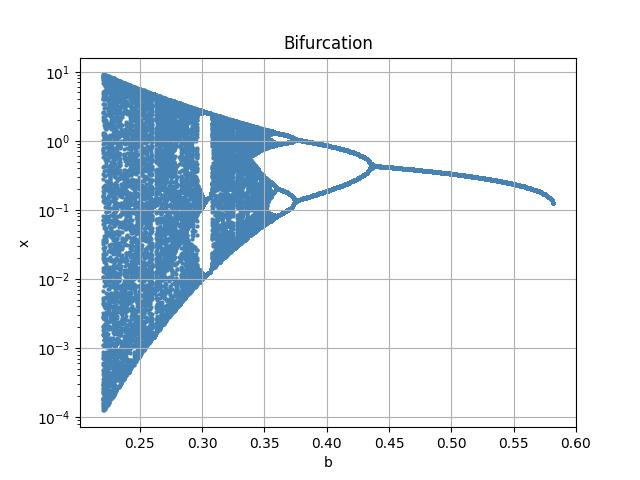
\includegraphics[width=0.55\textwidth]{stochastic/images/bifurcation_x_0_2_a_1_compare_no_noise.jpg}
            \label{bifurcation_x_0_2_a_1_compare_no_noise}
        }  
        \subfloat[для модели (\ref{alpha_chaos})]{
            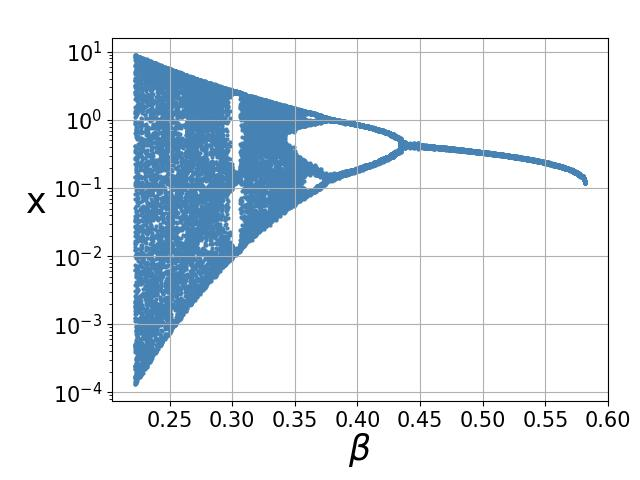
\includegraphics[width=0.55\textwidth]{stochastic/images/bifurcation_x_0_2_a_1_compare_alpha_noise.jpg}
            \label{bifurcation_x_0_2_a_1_compare_alpha_noise}
        }
        
        \subfloat[для модели (\ref{beta_chaos})]{
            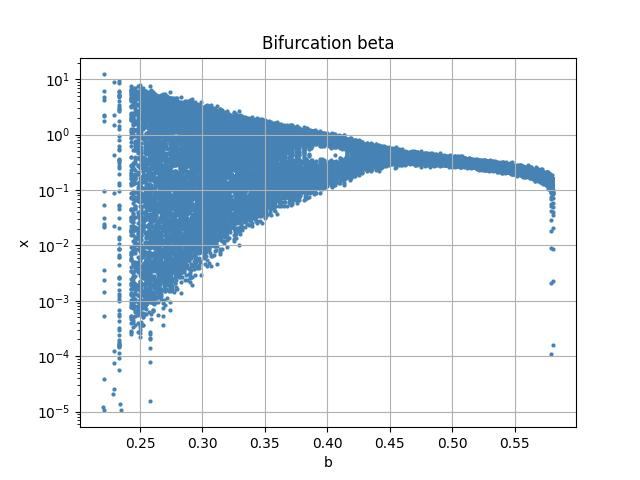
\includegraphics[width=0.55\textwidth]{stochastic/images/bifurcation_x_0_2_a_1_compare_beta_noise.jpg}
            \label{bifurcation_x_0_2_a_1_compare_beta_noise}
        }
        \subfloat[для модели (\ref{additive_chaos})]{
            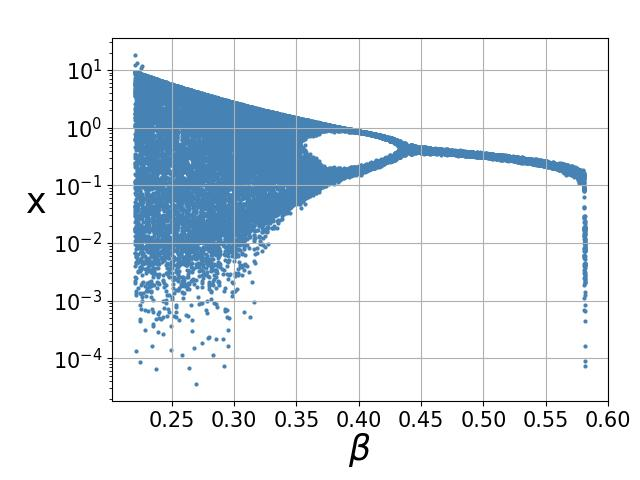
\includegraphics[width=0.55\textwidth]{stochastic/images/bifurcation_x_0_2_a_1_compare_additional_noise.jpg}
            \label{bifurcation_x_0_2_a_1_compare_additional_noise}
        }
            
        \caption{Бифуркационная диаграмма при \(\varepsilon = 0.01\)}
    \end{figure}

    % \begin{figure}
    %     \centering
    %     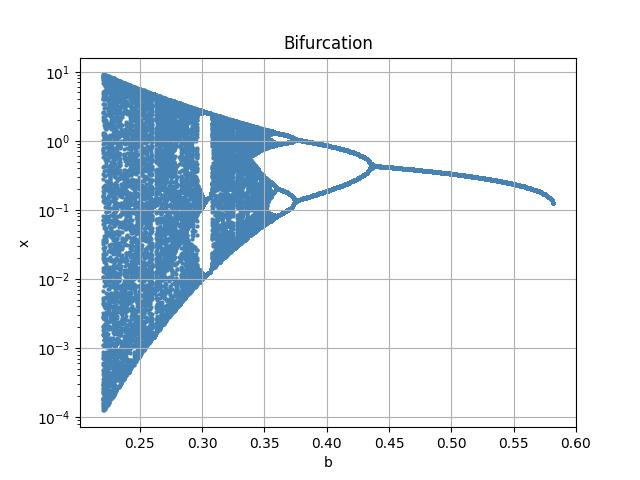
\includegraphics[width=\textwidth]{stochastic/images/bifurcation_x_0_2_a_1_compare_no_noise.jpg}
        
    %     \captionsetup{justification=centering}
    %     \caption{Бифуркационная диаграмма для модели (\ref{origin})}
    %     \label{bifurcation_x_0_2_a_1_compare_no_noise}
    % \end{figure}
